%-------------------------------------------------------------------------------
% 请勿删除本注释
% Free Response Question 2
%
% 指引:
% 如在小问之前有通用问题描述,请放置于此
%-------------------------------------------------------------------------------
\begin{figure}[H]
\centering
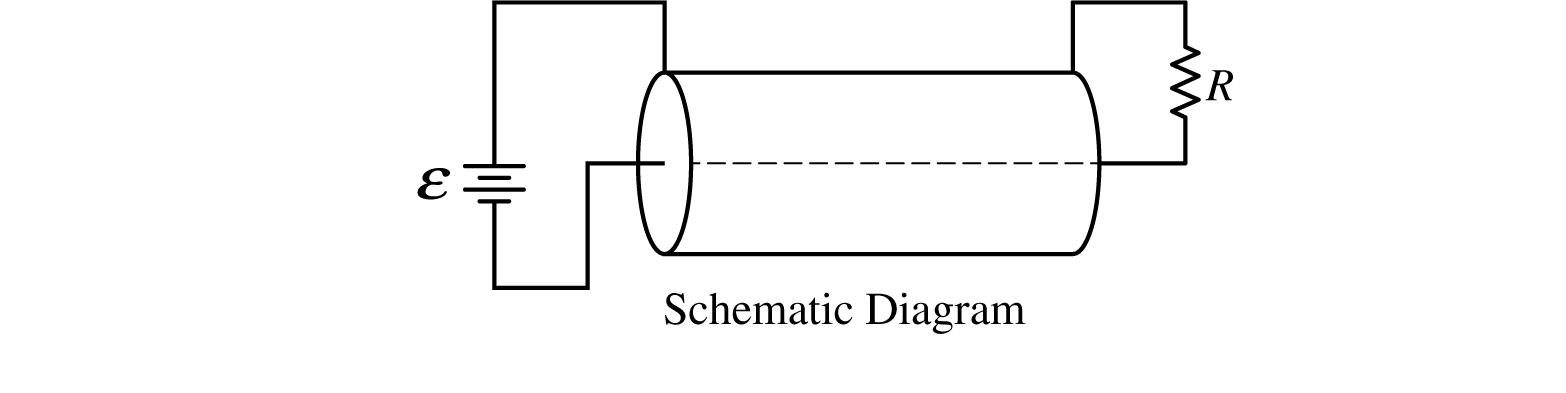
\includegraphics[scale=0.2]{images/img-022-037.png}
\end{figure}

\begin{figure}[H]
\centering
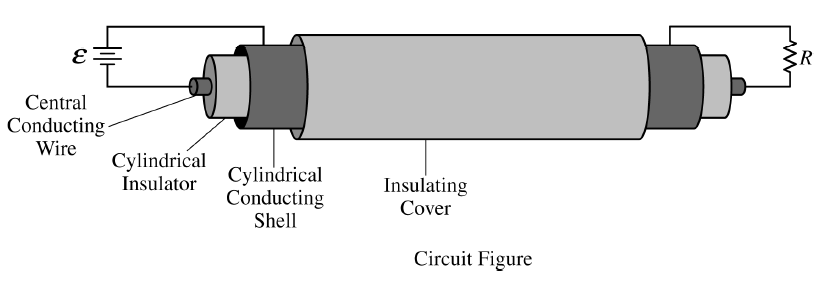
\includegraphics[scale=0.5]{images/2-a.png}
\end{figure}


\question
A coaxial cable is composed of a central conducting wire surrounded by a cylindrical insulator, and around that is a conducting cylindrical shell with an insulating cover. A power supply of emf $\varepsilon$ is used at one end to connect the two conducting regions, and a resistive load of resistance $R$ is connected at the other end of the cable to complete the circuit, as shown in the schematic diagram and circuit figure above. % 请删除并替换本行,与上一行 \question 之间不要留空行

\begin{figure}[H]
\centering
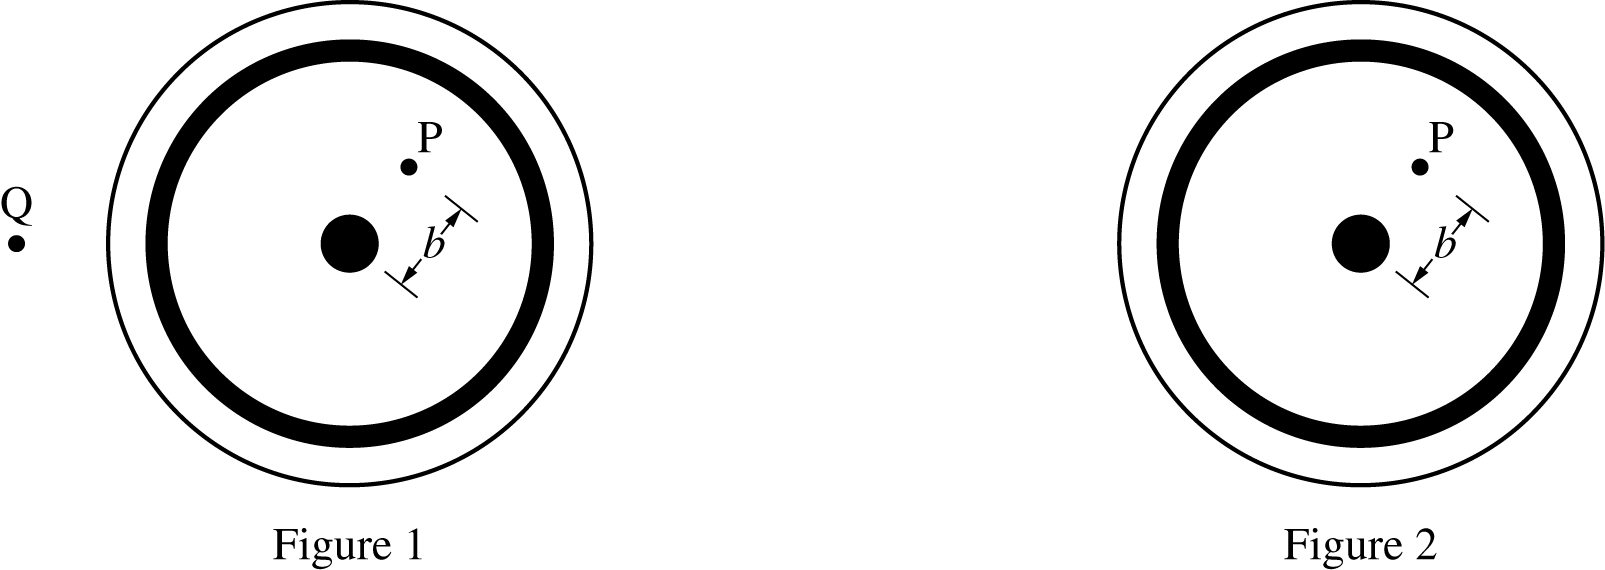
\includegraphics[scale=0.2]{images/img-022-039.png}
\end{figure}

A cross section of the cable from the perspective of the power supply end is depicted above as if looking into the left end of the cable. Point $\mathrm{P}$ is inside the cylindrical insulator a distance $b$ from the center of the cable. Point $\mathrm{Q}$ is outside the cable.

\begin{parts}

%-------------------------------------------------------------------------------
% 请勿删除本注释
% Part (a)
%
% 指引:
% 如在小问之前有通用问题描述,请放置于此
%-------------------------------------------------------------------------------

\part
 % 请删除并替换本行,与上一行 \part 之间不要留空行
\begin{subparts}
\subpart On figure 1 shown above left, draw an Amperian loop that could be used to determine the magnitude of the magnetic field at point P in the diagram. Clearly mark this loop as "Loop 1."
\subpart On figure 1, draw an Amperian loop that could be used to determine the magnitude of the magnetic field at point Q in the diagram. Clearly mark this loop as "Loop 2."
\subpart On figure 2 shown above right, draw an arrow to show the direction of the magnetic field at point P. The arrow should start on and point away from the point in the direction of the magnetic field.
\end{subparts}

%-------------------------------------------------------------------------------
% 请勿删除本注释
% Part (b)
%
% 指引:
% 如在小问之前有通用问题描述,请放置于此
%-------------------------------------------------------------------------------

\part
Using Ampere's law, derive an expression for the magnitude of the magnetic field at point P. Express your answer in terms of $\varepsilon, R, b$, and physical constants, as appropriate. % 请删除并替换本行,与上一行 \part 之间不要留空行

%-------------------------------------------------------------------------------
% 请勿删除本注释
% Part (c)
%
% 指引:
% 如在小问之前有通用问题描述,请放置于此
%-------------------------------------------------------------------------------

\part
Determine the magnitude of the magnetic field at point Q. % 请删除并替换本行,与上一行 \part 之间不要留空行

Justify your answer.

%-------------------------------------------------------------------------------
% 请勿删除本注释
% Part (d)
%
% 指引:
% 如在小问之前有通用问题描述,请放置于此
%-------------------------------------------------------------------------------

Some physics students conduct an experiment with a coaxial cable in which they connect the cable to a variable power supply and measure the resulting magnetic field strength at point P inside the cylindrical insulator using a magnetic field sensor. Point P is $0.0050 \mathrm{~m}$ from the center of the cable. The plot of the magnetic field strength $B$ as a function of the emf $\mathcal{E}$ of the power supply is shown below.

\begin{figure}[H]
\centering
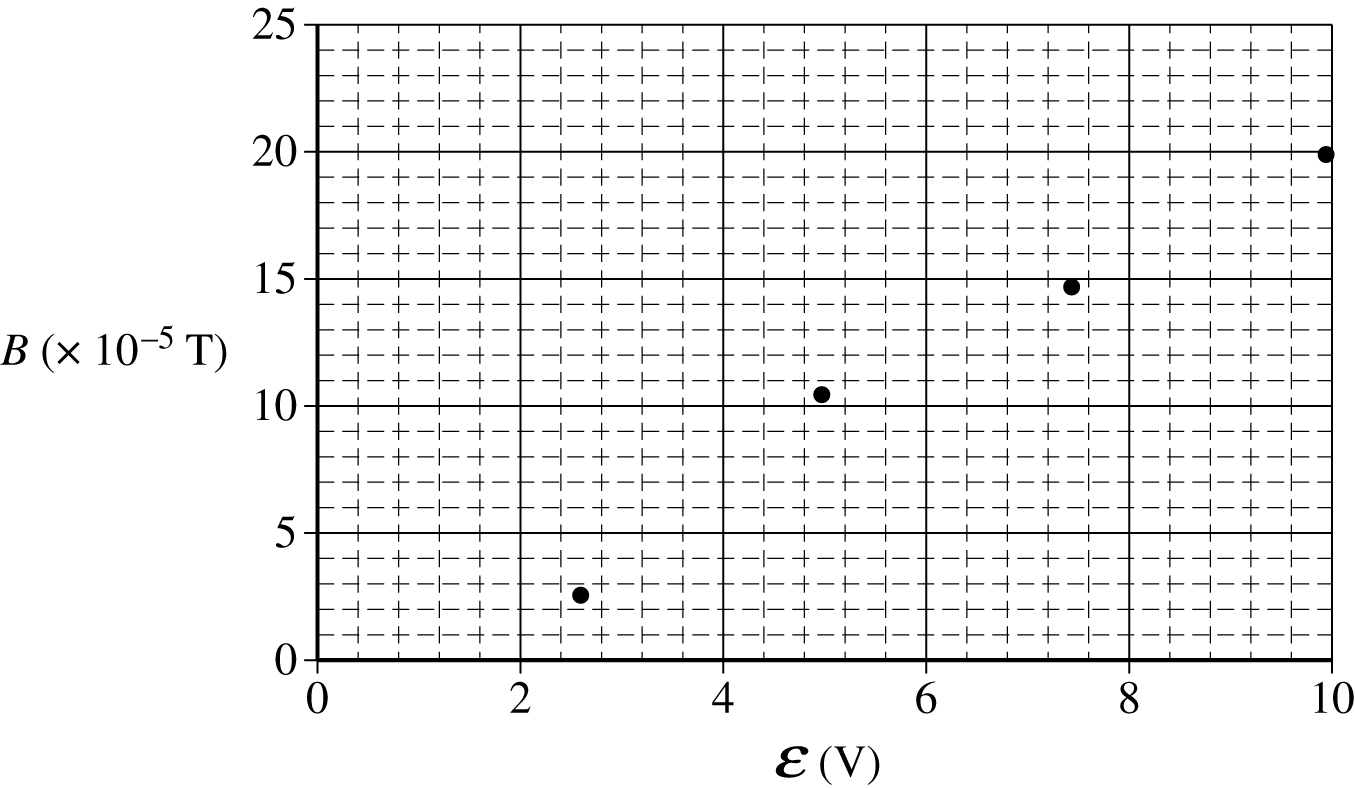
\includegraphics[scale=0.3]{images/img-024-040.png}
\end{figure}


\part
 % 请删除并替换本行,与上一行 \part 之间不要留空行
\begin{subparts}
\subpart Draw the best-fit line for the data.
\subpart Use the straight line to calculate the resistance $R$ of the resistor used in the experiment.
\end{subparts}

%-------------------------------------------------------------------------------
% 请勿删除本注释
% Part (e)
%
% 指引:
% 如在小问之前有通用问题描述,请放置于此
%-------------------------------------------------------------------------------

\part
The lab group uses a multimeter to measure the resistance of the resistor and determines that their experimental value for $R$ from part (d) is approximately $10 \%$ larger than that found with the multimeter. Describe a physical reason that might account for this result. % 请删除并替换本行,与上一行 \part 之间不要留空行

%-------------------------------------------------------------------------------
% 请勿删除本注释
% Part (f)
%
% 指引:
% 如在小问之前有通用问题描述,请放置于此
%-------------------------------------------------------------------------------

\part
The lab group notices that when the current is reversed in the cable and the experiment is again performed, the plot has a positive vertical axis intercept equal in magnitude to the negative vertical axis intercept in the plot shown before part (d). % 请删除并替换本行,与上一行 \part 之间不要留空行
\begin{subparts}
\subpart Describe a physical reason for the vertical axis intercept.
\subpart Describe a physical reason that the vertical axis intercept switches from negative to positive when the current in the cable is reversed.
\end{subparts}

\end{parts}
